\section{Piani di accesso}
\subsection{Piani di accesso logico}
Trovare tutti i commenti relativi ai modelli Ray-Ban.
\begin{center}
	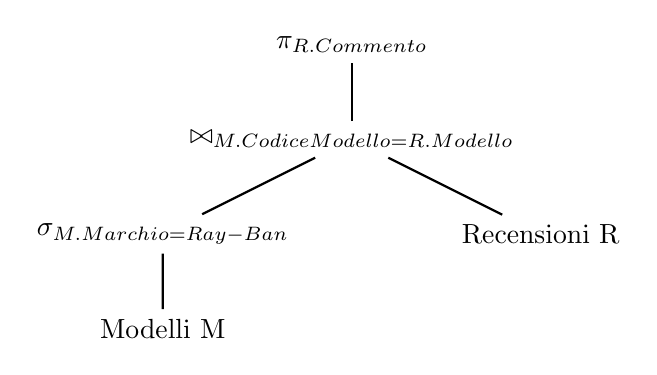
\begin{tikzpicture}[scale=0.8]
		\node (M) at (-3, 0) {Modelli M};
		\node (R) at (3, 1.5) {Recensioni R};
		\node (mrb) at (-3, 1.5) {$\sigma_\text{M.Marchio = Ray-Ban}$};
		\node (j) at (0, 3) {$\bowtie_\text{M.CodiceModello = R.Modello}$};
		\node (pc) at (0, 4.5) {$\pi_\text{R.Commento}$};

		\path (M) edge[thick] (mrb)
		(mrb) edge[thick] (j)
		(R) edge[thick] (j)
		(j) edge[thick] (pc);
	\end{tikzpicture}
\end{center}
Trovare tutte le categorie e i marchi che offrono occhiali di plastica tutti al di sotto dei 100
euro, ordinando dal più costoso al meno costoso.
\begin{center}
	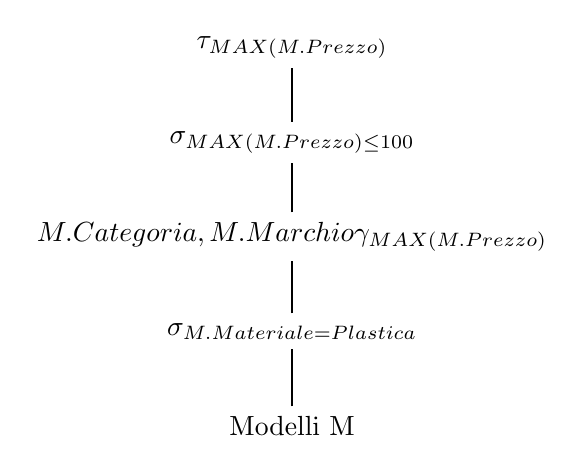
\begin{tikzpicture}[scale=0.8]
		\node (M) at (0, 0) {Modelli M};
		\node (plastica) at (0, 1.5) {$\sigma_\text{M.Materiale = Plastica}$};
		\node (group) at (0, 3) {$\prescript{}{\text{M.Categoria, M.Marchio}}{\gamma}_\text{MAX(M.Prezzo)}$};
		\node (having) at (0, 4.5) {$\sigma_{\text{MAX(M.Prezzo)} \leq 100}$};
		\node (order) at (0, 6) {$\tau_\text{MAX(M.Prezzo)}$};

		\path (M) edge[thick] (plastica);
		\path (plastica) edge[thick] (group);
		\path (group) edge[thick] (having);
		\path (having) edge[thick] (order);
	\end{tikzpicture}
\end{center}
Trovare il numero di modelli disponibile per ciascun colore di lenti che abbiano la montatura nera.
Non vengono visualizzati i colori di lenti applicati a meno di 10 modelli di occhiali.
\begin{center}
	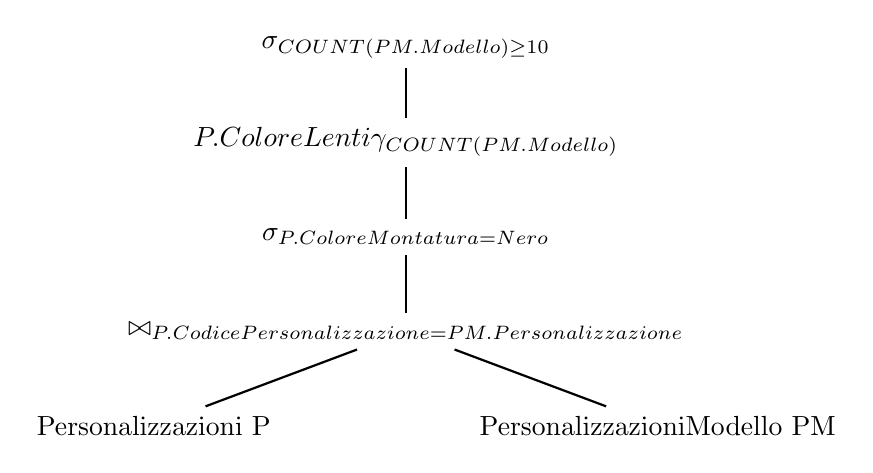
\begin{tikzpicture}[scale=0.8]
		\node (P) at (-4, 0) {Personalizzazioni P};
		\node (PM) at (4, 0) {PersonalizzazioniModello PM};
		\node (join) at (0, 1.5) {$\bowtie_\text{P.CodicePersonalizzazione = PM.Personalizzazione}$};
		\node (nero) at (0, 3) {$\sigma_\text{P.ColoreMontatura = Nero}$};
		\node (group) at (0, 4.5) {$\prescript{}{\text{P.ColoreLenti}}{\gamma}_\text{COUNT(PM.Modello)}$};
		\node (having) at (0, 6) {$\sigma_{\text{COUNT(PM.Modello)} \geq 10}$};

		\path (P) edge[thick] (join)
		(PM) edge[thick] (join)
		(join) edge[thick] (nero)
		(nero) edge[thick] (group)
		(group) edge[thick] (having);
	\end{tikzpicture}
\end{center}
\newpage

\subsection{Piani di accesso fisico senza indice}
Trovare tutti i commenti relativi ai modelli Ray-Ban.
\begin{center}
	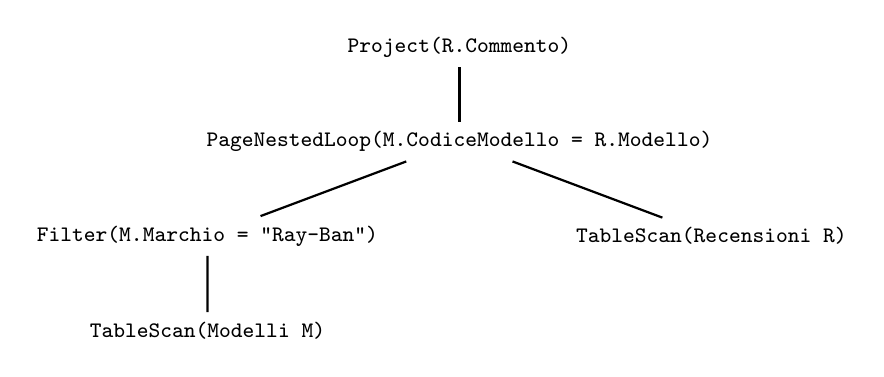
\begin{tikzpicture}[scale=0.8, font=\footnotesize]
		\node (M) at (-4, 0) {\verb|TableScan(Modelli M)|};
		\node (R) at (4, 1.5) {\verb|TableScan(Recensioni R)|};
		\node (mrb) at (-4, 1.5) {\verb|Filter(M.Marchio = "Ray-Ban")|};
		\node (j) at (0, 3) {\verb|PageNestedLoop(M.CodiceModello = R.Modello)|};
		\node (pc) at (0, 4.5) {\verb|Project(R.Commento)|};

		\path (M) edge[thick] (mrb)
		(mrb) edge[thick] (j)
		(R) edge[thick] (j)
		(j) edge[thick] (pc);
	\end{tikzpicture}
\end{center}
Trovare tutte le categorie e i marchi che offrono occhiali di plastica tutti al di sotto dei 100
euro, ordinando dal più costoso al meno costoso.
\begin{center}
	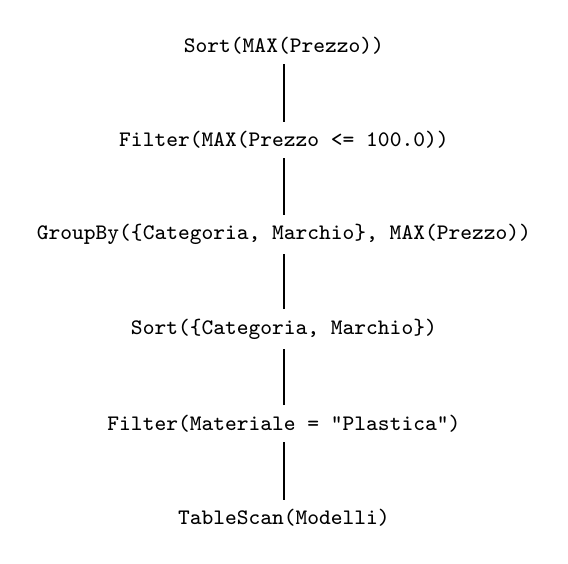
\begin{tikzpicture}[scale=0.8, font=\footnotesize]
		\node (M) at (0, 0) {\verb|TableScan(Modelli)|};
		\node (plastica) at (0, 1.5) {\verb|Filter(Materiale = "Plastica")|};
		\node (sort1) at (0, 3) {\verb|Sort({Categoria, Marchio})|};
		\node (group) at (0, 4.5) {\verb|GroupBy({Categoria, Marchio}, MAX(Prezzo))|};
		\node (having) at (0, 6) {\verb|Filter(MAX(Prezzo <= 100.0))|};
		\node (order) at (0, 7.5) {\verb|Sort(MAX(Prezzo))|};

		\path (M) edge[thick] (plastica);
		\path (plastica) edge[thick] (sort1);
		\path (sort1) edge[thick] (group);
		\path (group) edge[thick] (having);
		\path (having) edge[thick] (order);
	\end{tikzpicture}
\end{center}
Trovare il numero di modelli disponibile per ciascun colore di lenti che abbiano la montatura nera.
Non vengono visualizzati i colori di lenti applicati a meno di 10 modelli di occhiali.
\begin{center}
	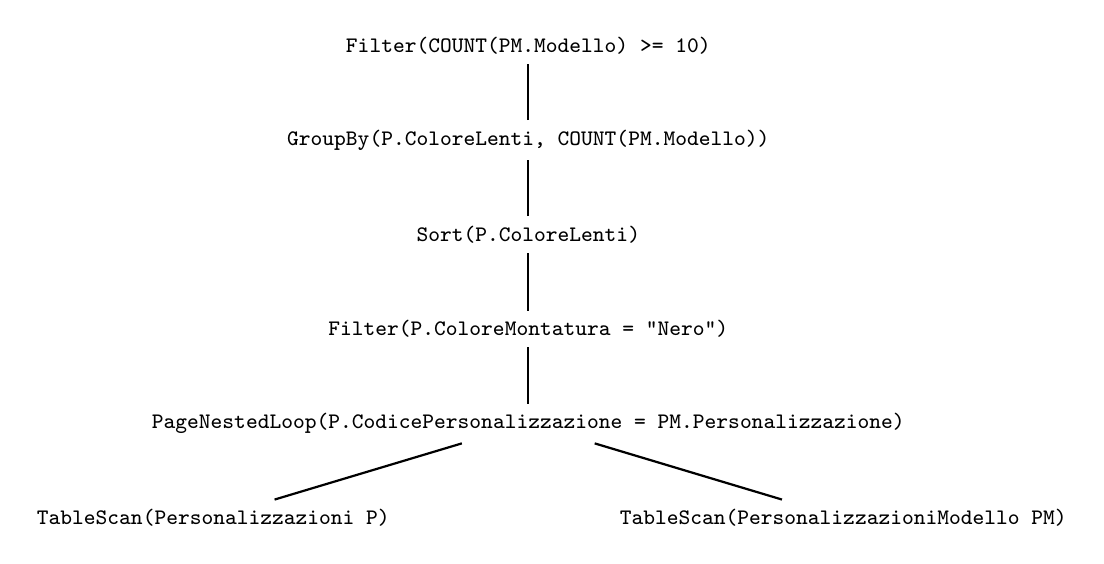
\begin{tikzpicture}[scale=0.8, font=\footnotesize]
		\node (P) at (-5, 0) {\verb|TableScan(Personalizzazioni P)|};
		\node (PM) at (5, 0) {\verb|TableScan(PersonalizzazioniModello PM)|};
		\node (join) at (0, 1.5) {\verb|PageNestedLoop(P.CodicePersonalizzazione = PM.Personalizzazione)|};
		\node (nero) at (0, 3) {\verb|Filter(P.ColoreMontatura = "Nero")|};
		\node (sort) at (0, 4.5) {\verb|Sort(P.ColoreLenti)|};
		\node (group) at (0, 6) {\verb|GroupBy(P.ColoreLenti, COUNT(PM.Modello))|};
		\node (having) at (0, 7.5) {\verb|Filter(COUNT(PM.Modello) >= 10)|};

		\path (P) edge[thick] (join)
		(PM) edge[thick] (join)
		(join) edge[thick] (nero)
		(nero) edge[thick] (sort)
		(sort) edge[thick] (group)
		(group) edge[thick] (having);
	\end{tikzpicture}
\end{center}

\subsection{Piani di accesso fisico con indice}
Trovare tutti i commenti relativi ai modelli Ray-Ban.
\begin{center}
	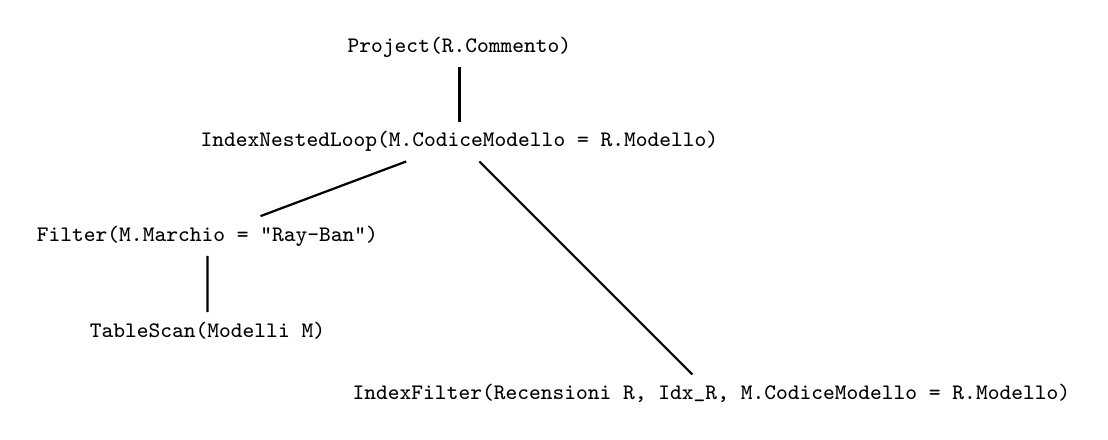
\begin{tikzpicture}[scale=0.8, font=\footnotesize]
		\node (M) at (-4, 0) {\verb|TableScan(Modelli M)|};
		\node (R) at (4, -1) {\verb|IndexFilter(Recensioni R, Idx_R, M.CodiceModello = R.Modello)|};
		\node (mrb) at (-4, 1.5) {\verb|Filter(M.Marchio = "Ray-Ban")|};
		\node (j) at (0, 3) {\verb|IndexNestedLoop(M.CodiceModello = R.Modello)|};
		\node (pc) at (0, 4.5) {\verb|Project(R.Commento)|};

		\path (M) edge[thick] (mrb)
		(mrb) edge[thick] (j)
		(R) edge[thick] (j)
		(j) edge[thick] (pc);
	\end{tikzpicture}
\end{center}
Trovare tutte le categorie e i marchi che offrono occhiali di plastica tutti al di sotto dei 100
euro, ordinando dal più costoso al meno costoso.
\begin{center}
	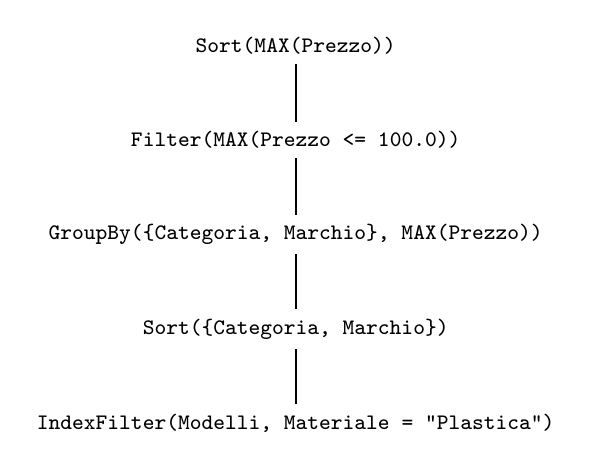
\begin{tikzpicture}[scale=0.8, font=\footnotesize]
		\node (plastica) at (0, 1.5) {\verb|IndexFilter(Modelli, Materiale = "Plastica")|};
		\node (sort1) at (0, 3) {\verb|Sort({Categoria, Marchio})|};
		\node (group) at (0, 4.5) {\verb|GroupBy({Categoria, Marchio}, MAX(Prezzo))|};
		\node (having) at (0, 6) {\verb|Filter(MAX(Prezzo <= 100.0))|};
		\node (order) at (0, 7.5) {\verb|Sort(MAX(Prezzo))|};

		\path (plastica) edge[thick] (sort1);
		\path (sort1) edge[thick] (group);
		\path (group) edge[thick] (having);
		\path (having) edge[thick] (order);
	\end{tikzpicture}
\end{center}
Trovare il numero di modelli disponibile per ciascun colore di lenti che abbiano la montatura nera.
Non vengono visualizzati i colori di lenti applicati a meno di 10 modelli di occhiali.
\begin{center}
	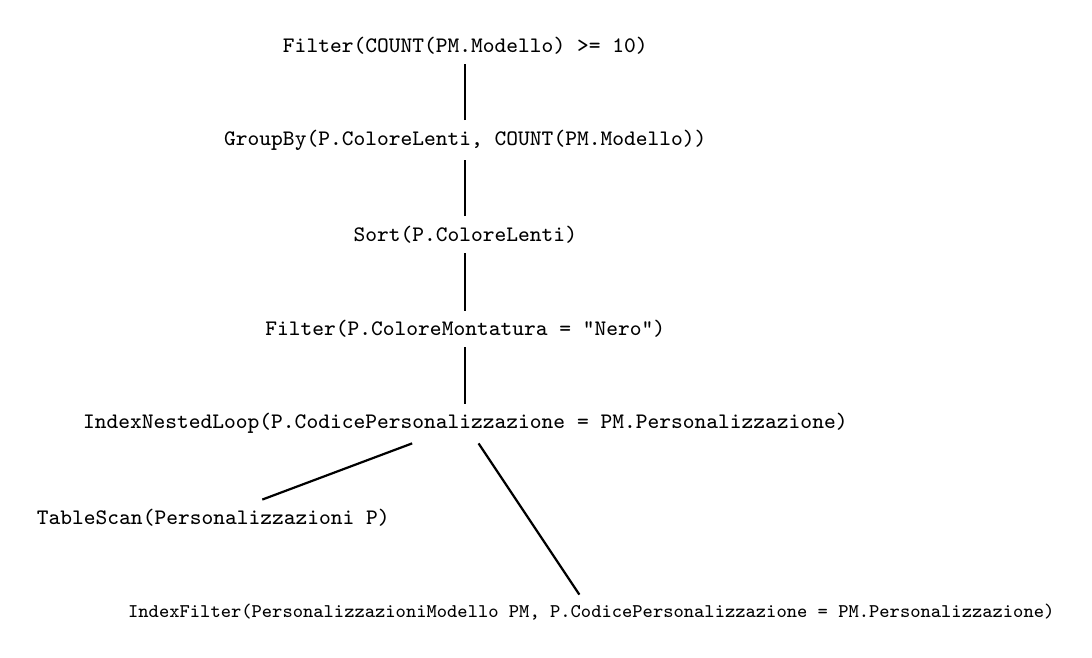
\begin{tikzpicture}[scale=0.8, font=\footnotesize]
		\node (P) at (-4, 0) {\verb|TableScan(Personalizzazioni P)|};
		\node (PM) at (2, -1.5) {\scriptsize\verb|IndexFilter(PersonalizzazioniModello PM, P.CodicePersonalizzazione = PM.Personalizzazione)|};
		\node (join) at (0, 1.5) {\verb|IndexNestedLoop(P.CodicePersonalizzazione = PM.Personalizzazione)|};
		\node (nero) at (0, 3) {\verb|Filter(P.ColoreMontatura = "Nero")|};
		\node (sort) at (0, 4.5) {\verb|Sort(P.ColoreLenti)|};
		\node (group) at (0, 6) {\verb|GroupBy(P.ColoreLenti, COUNT(PM.Modello))|};
		\node (having) at (0, 7.5) {\verb|Filter(COUNT(PM.Modello) >= 10)|};

		\path (P) edge[thick] (join)
		(PM) edge[thick] (join)
		(join) edge[thick] (nero)
		(nero) edge[thick] (sort)
		(sort) edge[thick] (group)
		(group) edge[thick] (having);
	\end{tikzpicture}
\end{center}
